\documentclass[submit,techreq,noauthor]{eco}	% semi style
\usepackage[dvips]{graphicx}
\usepackage{listings, jlisting} 		% for source code
\usepackage{url}
\usepackage{setspace}
\usepackage{here}
%\setstretch{1.5} % 行間を広くします(資料チェックしてもらうときはコメントを外す)
\lstset{
  basicstyle={\ttfamily},
  identifierstyle={\small},
  commentstyle={\smallitshape},
  keywordstyle={\small\bfseries},
  ndkeywordstyle={\small},
  stringstyle={\small\ttfamily},
  frame={tb},
  breaklines=true,
  columns=[l]{fullflexible},
  numbers=left,
  xrightmargin=0zw,
  xleftmargin=3zw,
  numberstyle={\scriptsize},
  stepnumber=1,
  numbersep=1zw,
  lineskip=-0.5ex
}

\begin{document}

\semino {4/10}					% 年度/回数
\date   {4/12/16/金}				% 平成/月/日/曜日
\title  {Expected Exploitability: Predicting the Development of Functional Vulnerability Exploits}	% タイトル
\author {山下 恭平}				% 氏名

\begin{abstract}
本稿は31st USENIX Security Symposiumにて掲載された論文「Expected Exploitability: Predicting 
the Development of Functional Vulnerability Exploits」\begin{math}^{[1]}\end{math}の内容に
ついてまとめたものである.既存の脆弱性評価基準の分析を通じて得られる結果は,その脆弱性が悪用されることを予測する
のには不十分であるため,ソフトウェア脆弱性の公開時の悪用可能性を評価することは困難である.さらに,「悪用できない」
という評価は不確実性が高く,悪用可能性の評価にはバイアスがかかっていることが問題として挙げられる.これらの問題を解決するために,機能的な
エクスプロイトが開発される可能性を経時的に反映する,Expected Exploitability(EE)と呼ばれる新しい指標を提案
する.

\end{abstract}
\maketitle

\section{はじめに}
エクスプロイトがセキュリティに深刻な影響を与えた事例として,2017年に世界中で大流行したWannaCryとNotPetya
がある.これらが悪名高い成功を納めた原因として,武器化されたエクスプロイトの使用が挙げられる.しかし,武器となり得る
脆弱性を利用するプログラムを開発する難易度が上がっていることから,既知の脆弱性のうち5\%のみを悪用することに注力
するようになっている.そういった中で,着目すべき脆弱性の優先順位をつけることで人々に対して最適な意思決定を
もたらし,悪用防止に向けた研究機会の深い理解のために,各脆弱性の悪用可能性を評価する必要がある.しかし,悪用可能性
の評価は,どの脆弱性が,どのように利用されるかが不明なため,困難である.具体的には,WannaCryやNotPetyaによって
悪用された脆弱性であるCVE-2017-0144は,当時の専門家が推奨するパッチから省かれたいた.このことから,エクスプロイト
の開発によってエクスプロイト可能性を証明することはできるが,非エクスプロイト可能性を証明することは困難である.
この結果,「悪用不可能」という評価にはバイアスが発生し,不確実性を持つことが分かる.\\
\indent この問題を解決するためにExpected Exploitability (EE)と呼ばれる新しい指標を提案する.
この指標は,脆弱性を「悪用可能」または「悪用不可能」と決定的に分類するのではなく,類似の
脆弱性に関する過去のパターンに基づいて,機能的なエクスプロイトが開発される可能性を時系列で
継続的に推定するものである.ここで機能的なエクスプロイトとは,脆弱性が引き起こすセキュリティ
上の問題を完全に実現し,実際の攻撃を容易にするものである.本稿では,2章で
研究の背景と目的について述べ,3章では開発にあたっての課題について,4章では実際に取集するデータについてまとめ,
5章でEEの評価を行い,6章でそれらをまとめる.

\section{研究の背景と目的}

\subsection*{既存の評価についての問題}
エクスプロイトの開発によって,悪用可能性を証明することができるが,悪用不可能であることを
証明するのは困難である.その代わりに,脆弱性悪用緩和の取り組みとして,悪用の難しさを
把握することを目的とした脆弱性スコアリングシステムがよく用いられる.以下にその例をあげる.
\begin{quote}
  \begin{itemize}
   \item NVD CVSS\begin{math}^{[2]}\end{math}
    \begin{itemize}
      \item 脆弱性を悪用することの容易さと技術的手段を反映することを目的とした,悪用可能性の評価指標を持つスコアリングシステム.必要なアクセス数,攻撃の複雑さ,権限レベルなど,様々な脆弱性の特性を0〜4の数値に落とし込んだもの.
    \end{itemize}
   \item Microsoft Exploitability Index\begin{math}^{[3]}\end{math}
    \begin{itemize}
      \item Microsoftが0〜3の4段階で悪用可能性を評価し割り当てる,Microsoft固有のスコア.
    \end{itemize}
   \item RedHat Severity\begin{math}^{[4]}\end{math}
    \begin{itemize}
      \item CVSSを補完し,RedHat製品に影響を与える脆弱性について専門家の評価によって,同様に脆弱性の悪用の難易度を評価したもの.
    \end{itemize}
  \end{itemize}
\end{quote}

\begin{figure}[H]
  \centering
  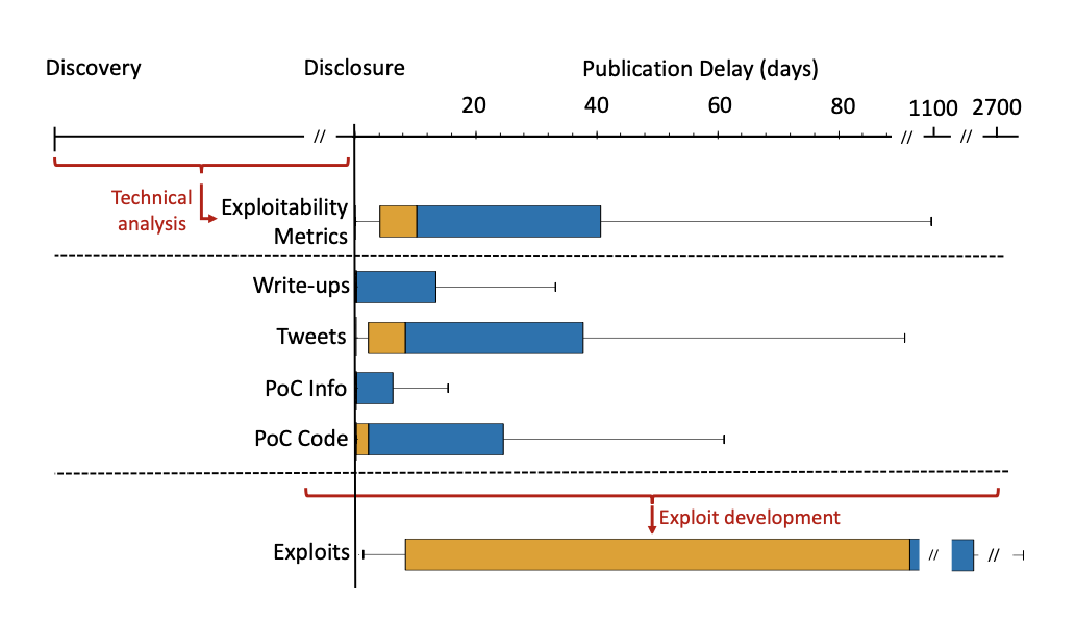
\includegraphics[scale=0.4]{fig/pic1.eps}
  \caption{脆弱性情報のタイムライン}
\end{figure}

しかし,これらのベンダーなどから提供される指標は,不正確であることが報告されている.
具体的な事例として,Internet Explorerの悪用可能な脆弱性であるCVE-2018-8174は,CVSS
悪用可能性スコア1.6を獲得し,脆弱性スコアの91\%以下に位置づけられた.同様に,Windows7
から10に影響を及ぼす悪用をされる脆弱性であるCVE-2018-8440は,スコアが1.8とされた.これらの
指標が悪用可能性を適切に反映できない原因を説明するために,図1に典型的な脆弱性のタイム
ラインを示す.これらの指標は,脆弱性が公開される前に行われる技術的分析によって定める.
しかし,脆弱性の公開後,脆弱性に関する追加の技術情報やPoCなどの様々な脆弱性
の成果物が公開され,それらについてSNSなどで議論が行われることが観察された.これらの
成果物から悪用の可能性についての有益な情報が得られることがよく発生する.CVE-2018-8174
は技術的なWrite-upの公開がエクスプロイトの開発の直接的な原因になったと報告されており,
CVE-2018-8440のPoCは2日以内に悪用を引き起こすと判断されている.これらの例は,
既存の指標が,公開後にのみ利用可能な有用なエクスプロイト情報を考慮できておらず,時間の
経過と共に更新されていないことを明らかにした.

\subsection*{研究の目的}
\indent このことから,悪用可能性の時間的な変化は,確立的なプロセスで記述できることが示唆される.
ある時点において,悪用可能性は悪用を観測する確率を符号化した確率変数Eと考えられ,悪用が不可能
とされている脆弱性には確率0を,悪用が確認されている脆弱性には1を割り当てる.しかし,Eを生成する
真の分布Eは利用不可能であり,実際はノイズを含めた\begin{math}E^{train}\end{math}を
使用する必要がある.これは,悪用可能性の期待値を推定する尤度を計算することによって,利用可能な
データからEを近似する必要があることを意味する.この指標のことをExpected Exploitability (EE)と呼ぶ.
EEは教師あり機械学習を用いて過去のデータから学習することができ,新しいエクスプロイトが開発,発見される前に
,脆弱性に対する悪用の可能性を評価することを可能にする.この研究の目的は,既知の脆弱性に対して機能するエクス
プロイトが開発されるかどうかを予測することで,その脆弱性の悪用可能性を客観的に定量化することである.

\section{EE開発の課題}
EEに教師あり機械学習の技術を適用するためには3つの課題がある.
ここでは,それぞれについて説明する.

\subsection*{PoCから特徴を抽出する}
PoCは脆弱性のトリガーとして設計されており,直接的な攻撃は行わない.しかし,機能的なエクスプロイトにおいて
必要なステップを満たしている.つまり,PoCコードの構造と複雑さは,脆弱性攻撃の難しさを直接反映すると考え
られる. PoCの持つ予測力を十分に活用するために,PoCの特徴を抽出することが求められる.しかし,PoCは
様々なプログラム言語で書かれており,コードと事由形式のテキストを組み合わせた物であることが多く,既存の
プログラム解析技術の適応が制限される.そのため,PoCの特徴抽出には,テキストとコードを分離し,有用なコード表現を
得るための新しい技術を必要とする.

\subsection*{ノイズの把握と軽減}
先行研究\begin{math}^{[14]}\end{math}によって,学習に利用できるラベルに偏りがあることが判明している.
この問題を機械学習におけるラベルノイズの問題と関連付ける試みはこれまで為されていない.さらに,エクスプロイト
の証拠を提供する個々のベンダーが,脆弱性のカバー率にばらつきがある.このような特徴に依存するノイズの問題はあ
まり研究されておらず,実世界のアプリケーションにおけるノイズの特徴を発見することは,機械学習における未解決の
問題と考えられる.このため,ラベルノイズの種類とその影響,およびそれに対処するための学習技術の設計が求められる.

\subsection*{時間的に変化する悪用可能性の評価}
脆弱性の公開後に出現する成果物は分類を向上させる可能性があるが,公開の遅れはタイムリーな予測の有用性に
影響を与える.そのため,EEの評価では,リアルタイム性と潜在性という両立困難な指標を使用する必要がある.

\section{収集するデータ}
機械学習に必要な特徴量を抽出するために,必要なデータを集める.以下は集めるデータの一覧である.

\subsection*{CVE ID}
CVE IDは最も広く普及し,相互参照されている公的な脆弱性識別システムの1つであるため,脆弱性を識別す
るためにCVE IDを使用する.

\subsection*{公開の脆弱性情報}
PoCがターゲットとする脆弱性に関する情報を,National Vulnerability Database(NVD)\begin{math}^{[5]}\end{math}から収集する.
NVDには,アナリストが収集した脆弱性情報が掲載されており,高度な技術的情報を得ることができる.各脆弱性に
対して利用可能な技術情報をより多く把握するために,いくつかの公開情報の参照も行う.以下に参照を行う公開情報の一覧を示す.
\begin{quote}
  \begin{itemize}
   \item Bugtraq\begin{math}^{[6]}\end{math}
   \item IBM X- Force Exchang\begin{math}^{[7]}\end{math}
   \item Vulners\begin{math}^{[8]}\end{math}
  \end{itemize}
\end{quote}
これらから278,297の文書、102,936の脆弱性を参照した.これらの文書は脆弱性に関して公開されている技術情報
の全体像を示すものであり,「write-up」と呼んでいる.

\subsection*{Proof of Concepts (PoCs)}
ExploitDB\begin{math}^{[9]}\end{math} ,  Bugtraq\begin{math}^{[6]}\end{math} ,  Vulners\begin{math}^{[8]}\end{math}
の3つのデータベースを参照し,公開PoCのデータ収集を行なった.重複した収集データは除去し,CVE IDにリンクされている48,709件のPoC
を対象とした.結果21,849件の異なる脆弱性に対応したPoCの収集に成功した.

\subsection*{SNSの情報}
2014年1月から2019年12月までの間にCVE IDに言及したツイートの収集を行なった.Twitter Filtered Stream API\begin{math}^{[10]}\end{math}
を用いて52,551件の脆弱性に関する140万のツイートを収集することに成功した.

\subsection*{開発済みのエクスプロイト情報}
開発済のエクスプロイトに関する包括的なデータセットがないため,複数の公開情報から証拠を集約した.以下は集約に使用した
公開情報一覧である.
\begin{quote}
  \begin{itemize}
   \item CVSS
   \item IBM X- Force Exchang\begin{math}^{[7]}\end{math}
   \item Bugtraq\begin{math}^{[6]}\end{math}
   \item Tenable Nessus\begin{math}^{[11]}\end{math}
   \item Skybox\begin{math}^{[12]}\end{math}
   \item AlienVault OTX\begin{math}^{[13]}\end{math}
  \end{itemize}
\end{quote}

\section{評価}
既存の2種類の悪用可能性予測であるEPSS\begin{math}^{[15]}\end{math}とSocial Media Classifier(SMC)
と比較を行ったところ.全ての実験において精度を上回った.また,時間によって精度が向上するのも確認された.また,
緊急性の高い脆弱性,重要な脆弱性についての実験も行い,結果,既存の評価指標よりも高い精度を得ることができた.
新しい指標
EEは次のurlで公開されており,CVE IDによって検索をかけ,実際の指標を閲覧することが可能である.\\\url{https://exploitability.app/}

\section{おわりに}
既存の脆弱性情報やエクスプロイトの情報など,様々な情報を取得し機械学習によって学習させ,悪用可能性を予測することに成功していた.
既存の指標は一度公開されると,更新されないことを問題にあげ,リアルタイム性が極めて高いシステムを開発していた.また,特徴量を
的確に抽出するための数学的思考やSNS文字列の分析など,多岐にわたる知見が使用されており,極めてレベルの高い研究だと感じた.
今後は,学習データのノイズをさらに減らすことで更なる精度を期待できると考えられる.

% 参考文献はここに記述
\begin{thebibliography}{99}
  \bibitem{main} Octavian Suciu , Connor Nelson , Zhuoer Lyu , Tiffany Bao , and Tudor Dumitras.
    \quad Expected Exploitability: Predicting the Development of Functional Vulnerability 
    Exploits. In 31th USENIX Security Symposium (USENIX Security 22), pages 377-394, 2022
    \bibitem{NVD CVSS}A complete guide to the common vulnerability scoring system.\\
      \url{https://www.first.org/cvss/v3.0/specification-document} . (15/12/2022)
    \bibitem{Microsoft}Microsoft exploitability index. Microsoft.\\
      \url{https://www.microsoft.com/en-us/msrc/exploitability-index} . (15/12/2022)
    \bibitem{Red Hat}Severity Rating. RedHat.\\
      \url{https://access.redhat.com/security/updates/classification/} . (15/12/2022)
    \bibitem{NVD}National vulnerability database.\\
      \url{https://nvd.nist.gov/} . (15/12/2022)
    \bibitem{Bugtraq}Bugtraq. Accenture.\\
      \url{https://bugtraq.securityfocus.com/archive} . (15/12/2022)
    \bibitem{IBM}IBM X- Force Exchang.\\
      \url{https://exchange.xforce.ibmcloud.com/} . (15/12/2022)
    \bibitem{Vulners}Vulners. Vulners vulnerability database.\\
      \url{https://vulners.com/} . (15/12/2022)
    \bibitem{ExploitDB}ExploitDB. The exploit database.\\
      \url{https://www.exploit-db.com/} . (15/12/2022)
    \bibitem{Twitter}Twitter. Filtered stream.\\
      \url{https://developer.twitter.com/en/docs/twitter-api/tweets/filtered-stream/introduction} . (15/12/2022)
    \bibitem{Nessus}Tenable Network Security. Nessus vulnerability scanner.\\
      \url{https://www.tenable.com/products/nessus} . (15/12/2022)
    \bibitem{Skybox}SkyBox. Vulnerability center.\\
      \url{https://www.vulnerabilitycenter.com/#home} . (15/12/2022)
    \bibitem{AlienVault}Alienvault otx. AlienVault.\\
      \url{https://otx.alienvault.com/} . (15/12/2022)
    \bibitem{classify}M. Bozorgi, L. K. Saul, S. Savage, and G. M. Voelker. Beyond heuristics: learning to classify vulnerabilities and predict exploits. In KDD, Washington, DC, Jul 2010.
    \bibitem{EPSS} J. Jacobs, S. Romanosky, B. Edwards, I. Adjerid, and M. Roytman. Exploit prediction scoring system (epss). Digital Threats: Research and Practice, 2(3), July 2021.
\end{thebibliography}

\end{document}
